%CHAPTER
\chapter{Návrh modulu}

%SECTION
\section{Vzhled dokumentu PDF}
\label{sec:navrh_vzhledu}
Při návrhu výsledného vzhledu celého dokumentu je potřeba klást důraz hlavně na co nejpřesnější transformaci webového formuláře do souboru PDF. Vzhled webového formuláře je zobrazen na obrázku \ref{fig:web_formular}.

%SUBSECTION
\subsection{Záhlaví}
Záhlaví dokumentu by mělo obsahovat jednoznačný identifikátor recenzního příspěvku doplněný o~název vědeckého příspěvku, který bude hodnocen. Rozhodně by zde nemělo chybět ani logo konference TSD (ideálně ve vektorovém formátu). V~případě, že název vědeckého příspěvku bude zasahovat do loga, bude název zkrácen na pevnou velikost.

%SUBSECTION
\subsection{Titulek}
Titulek dokumentu by měl uživateli jednoznačně říct, který vědecký příspěvek hodnotí (ideálně zobrazit název i identifikátor). Každý příspěvek má v~systému vlastní identifikátor (S-ID\#), stejně jako každý uživatel (U-ID\#) a samotné recenze (R-ID\#). V~titulku by nemělo chybět ani jméno recenzenta a doplňující informace týkající se vyplňování formuláře, případně recenzenta informovat o~nedostatcích a omezeních aktuálně vygenerovaného dokumentu PDF.

%SUBSECTION
\subsection{Formulář}
Vzhled formuláře by se měl v~ideálním případě shodovat s~webovým formulářem. První část formuláře obsahuje stupnicové hodnocení, zatímco druhá je spíše slovní formou. Po konzultaci s~vedoucím práce jsem se rozhodl, že kombinované pole reprezentující stupnicové hodnocení parametru bude nahrazeno skupinou přepínacích tlačítek. Důvody tohoto rozhodnutí spočívaly v~lepším zobrazení hodnot na stupnici a zároveň neschopností PHP generátorů zobrazit uživatelsky přívětivé kombinované pole. Pro uložení doplňujícího textu bylo použito textové pro případné poznámky ohledně stavu a obsahu vědeckého příspěvku. Element popisující \textit{Review state} (stav recenzního příspěvku) a tlačítko \textit{Save review} (uložit recenzní příspěvek) nebudou do formuláře vloženy, jejich funkce není potřebná pro modulem vytvářený formulář.

%SUBSECTION
\subsection{Hodnocený vědecký příspěvek}
Vygenerovaný dokument by měl hlavně sloužit pro vyplňování hodnotícího formuláře off-line a ideálně by měl obsahovat i veškerý obsah hodnoceného vědeckého příspěvku, aby měl recenzent možnost kdykoliv nahlédnout na jeho obsah. Tento příspěvek bude vložen na konec souboru PDF.

%SUBSECTION
\subsection{Vodoznak}
Často se stává, že se neoprávněně kopírují již hotová díla a vydávají se pod cizím jménem, proto je vhodné do celého dokumentu vložit vodoznak, který bude jasně říkat, že se jedná pouze o~ soubor v~recenzním řízení, nikoliv o~plnohodnotné dílo.

%SUBSECTION
\subsection{Fonty}
\label{subsec:fonty}
V~prostředí PDF a PostScript se lze setkat s~pojmem čtrnáct standardních/základních fontů. Tento pojem byl odvozen ze standardních třinácti PostScript fontů a vyjadřuje základní fonty používané při vytváření veškerých souborů PDF. Všechny základní fonty lze nalézt v~tabulce \ref{tab:table_basic_fonts}.

\begin{table}[h!]
\centering
\begin{tabular}{|l|l|} 
\hline
\textbf{Rodina fontů} & \textbf{Fonty}                                                                                               \\ 
\hline
\textit{Times}        & \begin{tabular}[c]{@{}l@{}}Times-Roman\\Times-Italic\\Times-Bold\\Times-BoldItalic\end{tabular}              \\ 
\hline
\textit{Helvetica}    & \begin{tabular}[c]{@{}l@{}}Helvetica\\Helvetica-Oblique\\Helvetica-Bold\\Helvetica-BoldOblique\end{tabular}  \\ 
\hline
\textit{Courier}      & \begin{tabular}[c]{@{}l@{}}Courier\\Courier-Oblique\\Courier-Bold\\Courier-BoldOblique\end{tabular}          \\ 
\hline
\textit{Symbol}       & Symbol                                                                                                       \\
\hline
\textit{ZapfDingbats}       & ZapfDingbats                      \\
\hline
\end{tabular}
\caption{Tabulka základních fontů v~souborech PDF
\label{tab:table_basic_fonts}}
\end{table}

\begin{figure}[h!]
\centering
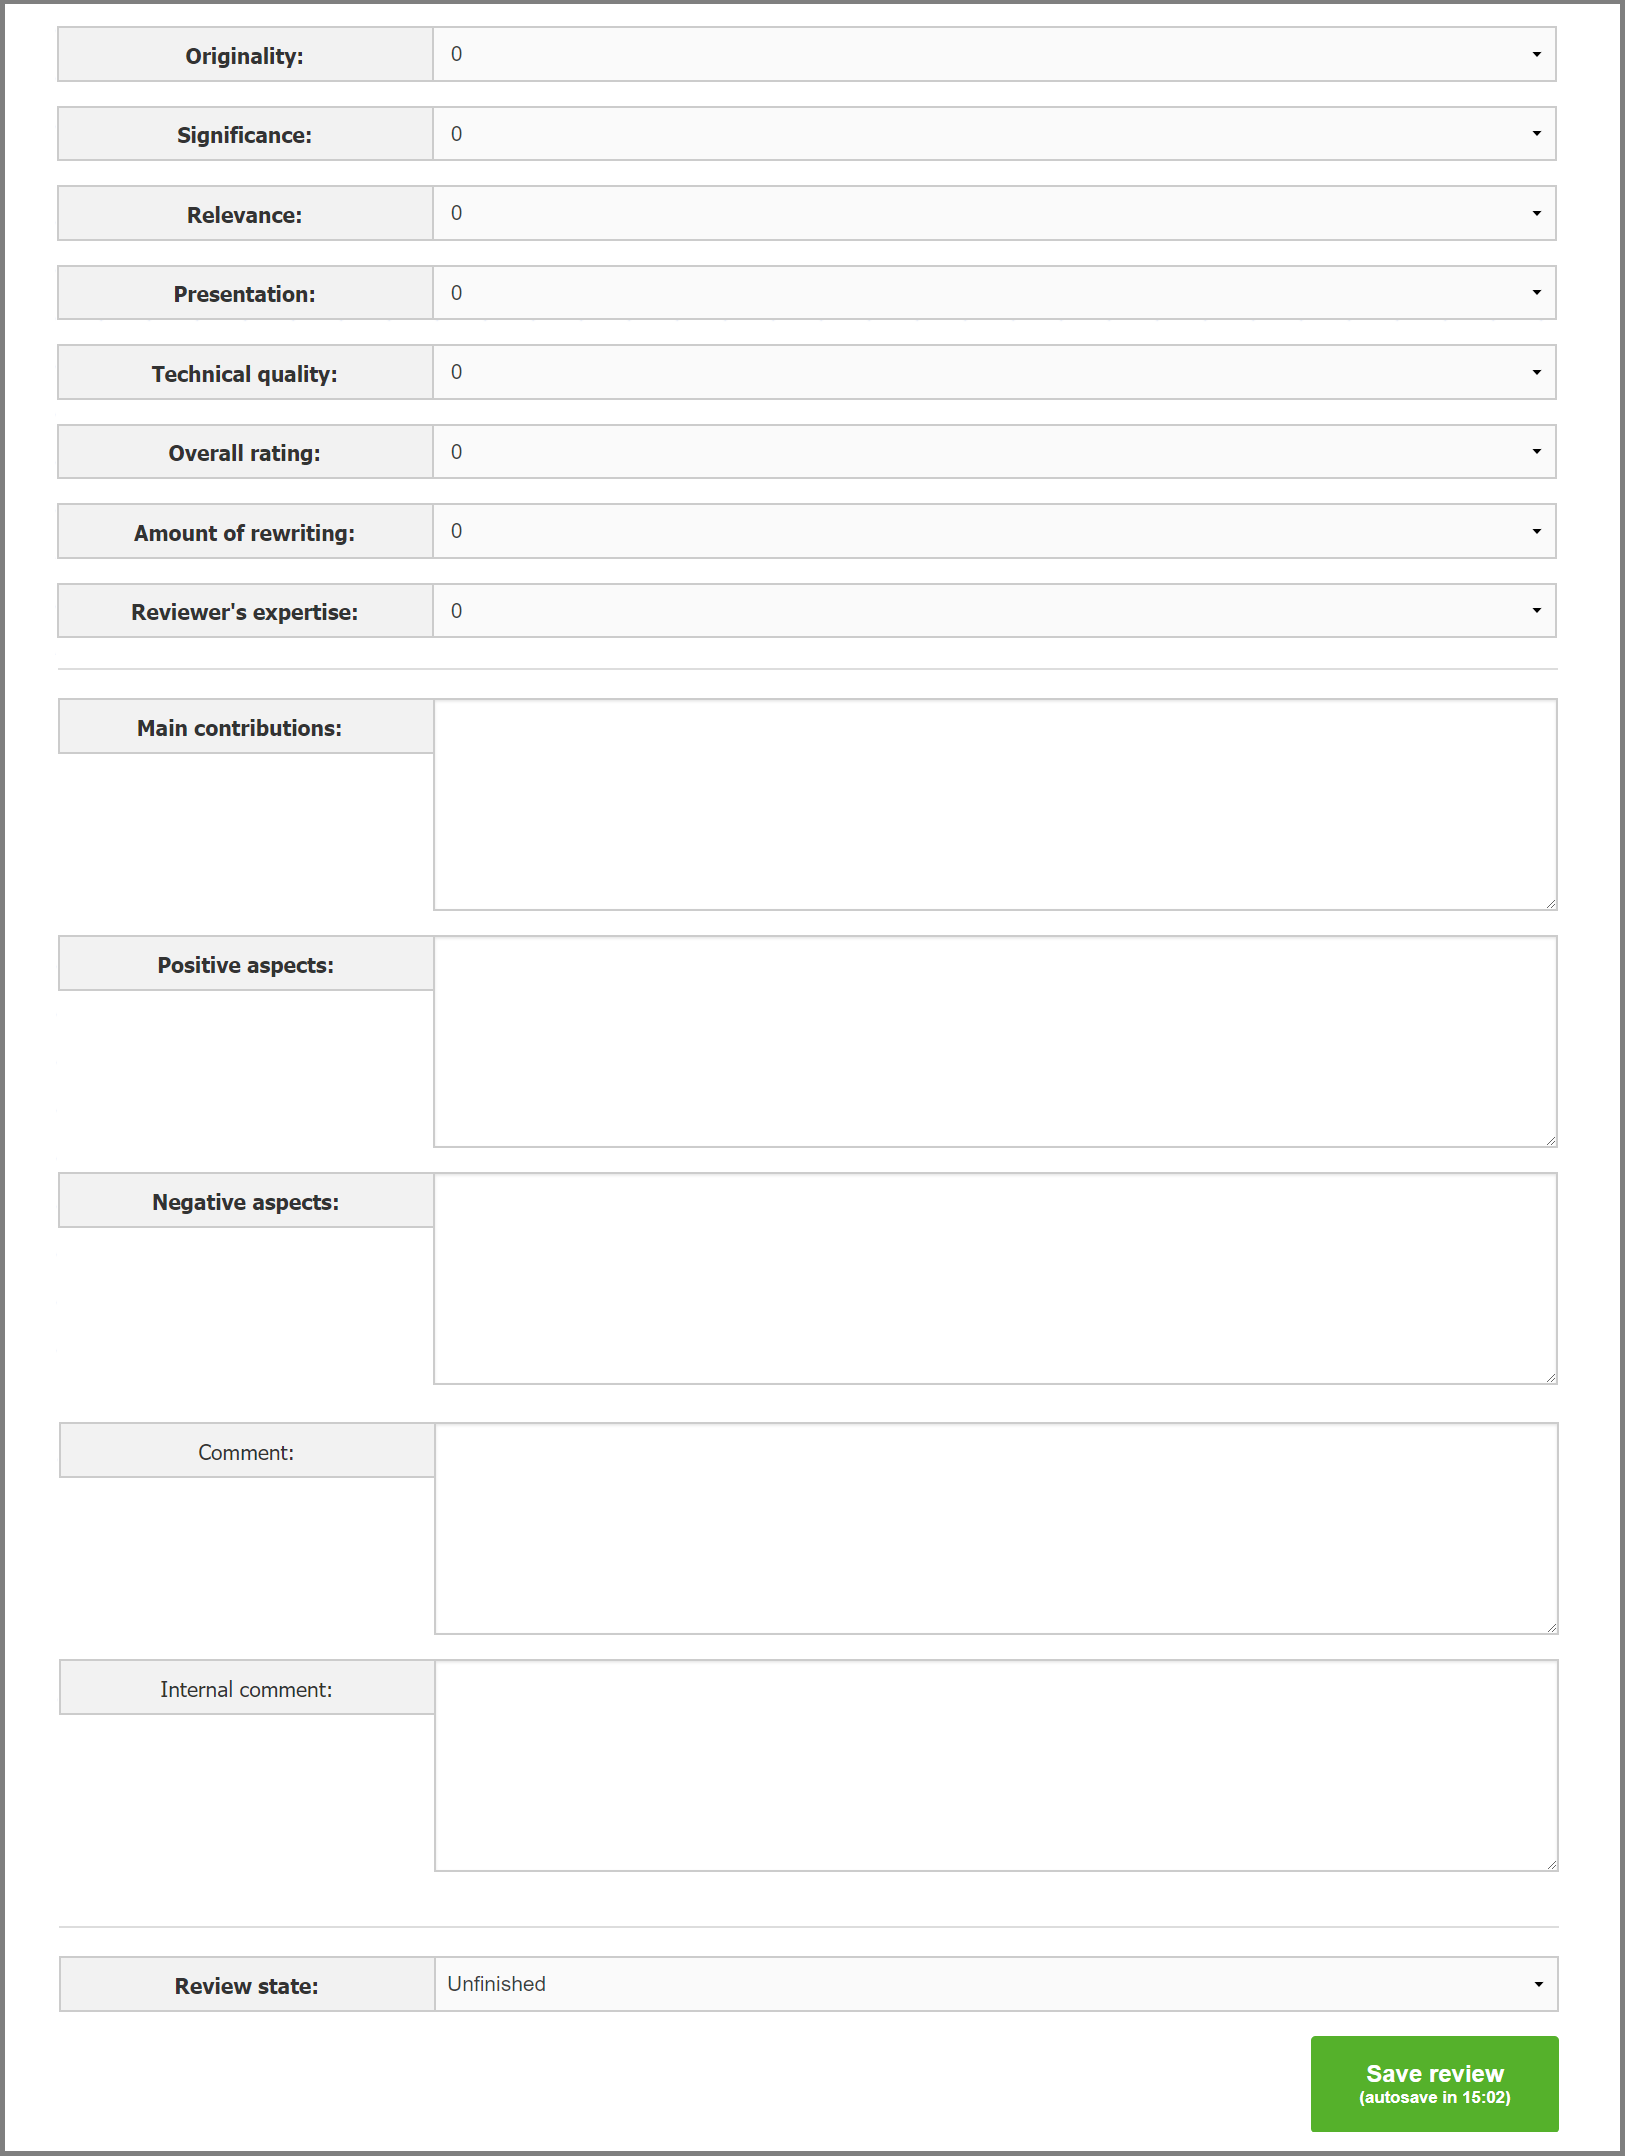
\includegraphics[width=15cm]{img/web_formular}
\caption{Webový formulář používaný pro hodnocení vědeckých příspěvků na portálu konference TSD}
\label{fig:web_formular}
\end{figure}

%SECTION
\section{Hlavní funkce modulu}
Vyvíjený modul musí být napsán stejným stylem jako je celý webový portál konferenčního systému TSD. Jelikož se na tomto portálu vyskytuje modul, který má stejnou funkcionalitu jako modul vyvíjený autorem bakalářské práce, tak je návrh funkcí jednodušší. Modul vyskytující se na portálu implementuje tři důležité funkce, které zajišťují veškerou funkcionalitu i přes to, že pro zpracovávání souborů PDF je použit externí program \textit{PDFtk}. Po konzultaci s~vedoucím práce bylo rozhodnuto, že se původní názvy funkcí zachovají a budou pouze změněny jejich parametry. Autorův modul bude tedy ve výsledku obsahovat, stejně jako starý modul, tři důležité funkce doplněny o~pomocné funkce a konstanty. Všechny hlavní funkce jsou popsány níže.  

%SUBSECTION
\subsection{Funkce pro generování}
Pro generování souboru PDF byla navržena jedna funkce. Tato funkce má za úkol nejdříve nastavit veškeré fonty a styly pro vzhled dokumentu, následně využít vhodný generátor souborů  PDF, který vytvoří všechny části dokumentu (vypsané v~kapitole \ref{sec:navrh_vzhledu}) a nabídne uživateli možnost stáhnout si výsledný soubor PDF v~recenzním řízení. Návrh hlavičky funkce viz výpis \ref{lst:generate_function}.

\lstset{style=phpstyle}
\begin{lstlisting}[caption = {Návrh hlavičky funkce pro generování souboru PDF}, label = {lst:generate_function}, captionpos=b]
function generate_offline_review_form($rid, $reviewer_name, $sid, $submission_name, $submission_filename)
\end{lstlisting}
Popis vstupních parametrů funkce:
\begin{itemize}
	\item\verb|$rid| -- ID hodnotícího příspěvku
	\item\verb|$reviewer_name| -- celé jméno recenzenta
	\item\verb|$sid| -- ID vědeckého příspěvku
	\item\verb|$submission_name| -- celý název vědeckého příspěvku
	\item\verb|$submission_filename| -- celý název souboru PDF vědeckého příspěvku
\end{itemize}

%SUBSECTION
\subsection{Funkce pro zpracování}
Pro zpracování souboru PDF byly navrženy dvě funkce, kdy první z~nich má za úkol nahrát celý soubor do konferenčního souboru. Po nahrání souboru začne extrakce dat pomocí vhodných parserů a zpracování vstupních souborů. Následně se vše uloží do odpovídajících struktur vícerozměrných polí a všechny extrahované hodnotící parametry se předají do následující funkce. Návrh hlavičky funkce viz výpis \ref{lst:process_function}.

\begin{lstlisting}[caption = {Návrh hlavičky funkce pro extrakci dat}, label = {lst:process_function}, captionpos=b]
function process_offline_review_form($rid, $sid, $revform_filename)
\end{lstlisting}
Popis vstupních parametrů funkce:
\begin{itemize}
	\item\verb|$rid| -- ID příspěvku v~recenzním řízení
	\item\verb|$sid| -- ID vědeckého příspěvku
	\item\verb|$revform_filename| -- celý název souboru PDF příspěvku v~recenzním řízení
\end{itemize}

Druhá funkce pro zpracování souboru PDF má za úkol uložit již extrahované hodnotící parametry do databáze konferenčního systému. Návrh hlavičky funkce viz výpis \ref{lst:upload_function}.

\begin{lstlisting}[caption = {Návrh hlavičky funkce pro uložení dat do databáze}, label = {lst:upload_function}, captionpos=b]
function upload_to_DB_offline_review_form($rid, $values)
\end{lstlisting}
Popis vstupních parametrů funkce:
\begin{itemize}
	\item\verb|$rid| -- ID příspěvku v~recenzním řízení
	\item\verb|$values| -- seznam všech hodnotících parametrů 
\end{itemize}